\def\year{2017}\relax
%File: formatting-instruction.tex
\documentclass[letterpaper]{article}
\usepackage{aaai17}
\usepackage{times}
\usepackage{helvet}
\usepackage{courier}
\usepackage{booktabs}
\usepackage{graphicx}
\frenchspacing
\setlength{\pdfpagewidth}{8.5in}
\setlength{\pdfpageheight}{11in}
\pdfinfo{
/Title (Comparative Analysis of Key Inference Methods from Monophonic Melodies in Symbolic Pop Music)
/Author (Paul M. Bodily, Dan Ventura)}
\setcounter{secnumdepth}{0}  
 \begin{document}
% The file aaai.sty is the style file for AAAI Press 
% proceedings, working notes, and technical reports.
%
\title{Comparative Analysis of Key Inference Methods from Monophonic Melodies in Symbolic Pop Music}
\author{Submission 2830}
%\author{Paul M. Bodily and Dan Ventura\\
%Department of Computer Science\\
%Brigham Young University\\
%Provo, UT 84602-6576\\
%}
\maketitle
\begin{abstract}
%Background
Key inference, a relatively simple task for trained human experts, is fundamental to analyzing melodic composition and prerequisite to normalizing musical data.
%Methods
We assess the accuracy of several traditional and machine learning approaches to the key inference problem on a dataset of 480 melodies in MIDI format. We evaluate the impact of including note duration and note repetition as learning features.
%Results
We find machine learning approaches outperform traditional key inference methods. The highest accuracies (0.729 for key inference and 0.896 for key signature inference) was achieved using a 4-gram language model.
%Conclusions
Including note duration improved the results of traditional approaches when inferring key, but had the opposite effect for key signature inference. Our findings suggest that the key of a melodic passage depends more heavily on the sequence of the notes rather than their frequency or distribution. 
\end{abstract}

\section{Introduction}

\noindent The key or tonic is a root pitch and modality (major or minor) which forms the structural basis for tonal music. This tonality provides a context within which ``the melodic and harmonic unfolding of a composition takes place'' \cite{vos1996parallel}. Even the untrained ear appreciates the structure, dissonance, and resolution that tonality provides.

Western pop music in particular presents an interesting case study because unlike much of its classical counterpart, pop songs regularly and deliberately break rules of traditional modulation and are often found to end on chords that are either unresolved or are entirely unrelated to the key in which the rest of the song is written.

There is a profound irony in the contrast between knowing how and being able to explain how to infer a song's key. Expert musicians routinely and accurately infer a song's key. However the best description for their methodology often goes no further than to find the key that ``feels'' right, provides a sense of ``finish'', or the key where the song ``lands''.

In this context it has commonly been supposed that one need simply find the key which minimizes the total number of accidentals in a song. Part of our purpose is to test this hypothesis by comparing this approach with several machine learning algorithms.

Harmony plays an integral role in determining a song's key. However, we hypothesize that the melody alone is sufficient in most cases to determine a song's key. We test this hypothesis on a dataset of 480 pop melodies in MIDI format.

\section{Related Work}

Several previous studies have examined key inference in various contexts, though to our knowledge our is the first attempt to do so using solely melodies and in the pop music domain.

Krumhansl matches the relative frequencies and durations with which tones are sounded (which she terms a \emph{tonal hierarchy}) of a song against the known tonal hierarchies of each key \cite{krumhansl2001cognitive}. This algorithm was applied to infer keys for compositions from three classical composers, Bach, Chopin, and Shostakovich. 

The key-finding algorithm of Longuet-Higgins and Steedman successively eliminates keys based on the presence or absence of the song's notes in each of the major and minor scales \cite{longuet1971interpreting}. Holtzman (1977) infers key from the prevalence of common key-defining intervals (e.g., triads, tonic-fifths, tonic-thirds). Both algorithms applied their algorithm to Bach's \emph{Well-Tempered Clavier}.

Hu and Saul take an LDA approach to key-finding, looking for common co-occurrences of notes in songs. Their model essentially treats keys like topics. They then model songs as a random mixture of key-profiles, allowing them to track modulations \cite{hu2009probabilistic}. Temperley interprets the traditional key-profile model as a Bayesian probabilistic model and discusses the implications of the connection between these two models \cite{temperley2002bayesian}. All applications of the model are on the Kostka-Payne corpus, a collection of textbook excerpts of tonal music. Vos and Van Geenen present a parallel search key-finding algorithm for single-voiced music. A song's notes are evaluated against both the scalar and the chordal structures of each key. They demonstrate the model's effectiveness on Bach's Well-Tempered Clavier \cite{vos1996parallel}. Zhu et al. present a method for key estimation in acoustic pop and classical music \cite{zhu2005music}. Their method performs marginally higher with pop music than classical music. 

Much recent work has been devoted to inferring key from acoustic music. Shenoy et al. outline a rule-based algorithm for finding key from acoustic musical signals using chroma based frequency analysis and chord progression patterns \cite{shenoy2004key}. Mauch and Dixon infer chords and key simultaneously from audio \cite{mauch2010simultaneous}. Chafe et al. extract symbolic music from audio from which meter and key are inferred (in that order) \cite{chafe1982toward}. The key-recognizer assumes that rhythmic and melodic accent points are significant features for inferring key.

Several methods have been presented for identifying key signature. They have been used mostly in Classical music. Pop music uses different modulations and is unique in that often the song finishes on a chord other than the key the song is in. No studies were found to examine key inference in pop melodies.

\section{Methods}

\subsection{Data}

We collected 480 melodies from 278 pop artists representing music spanning several decades (see Figure~\ref{tab:data_summary}). Songs were compiled from several online MIDI databases and keys were manually labeled. We were pleased to find that every key was represented by at least two songs (see Figure~\ref{fig:key_distribution}). Only songs with a single key were selected for our experiments. Melodies notes were isolated from the MIDI files. 


\begin{figure}
  \centering
 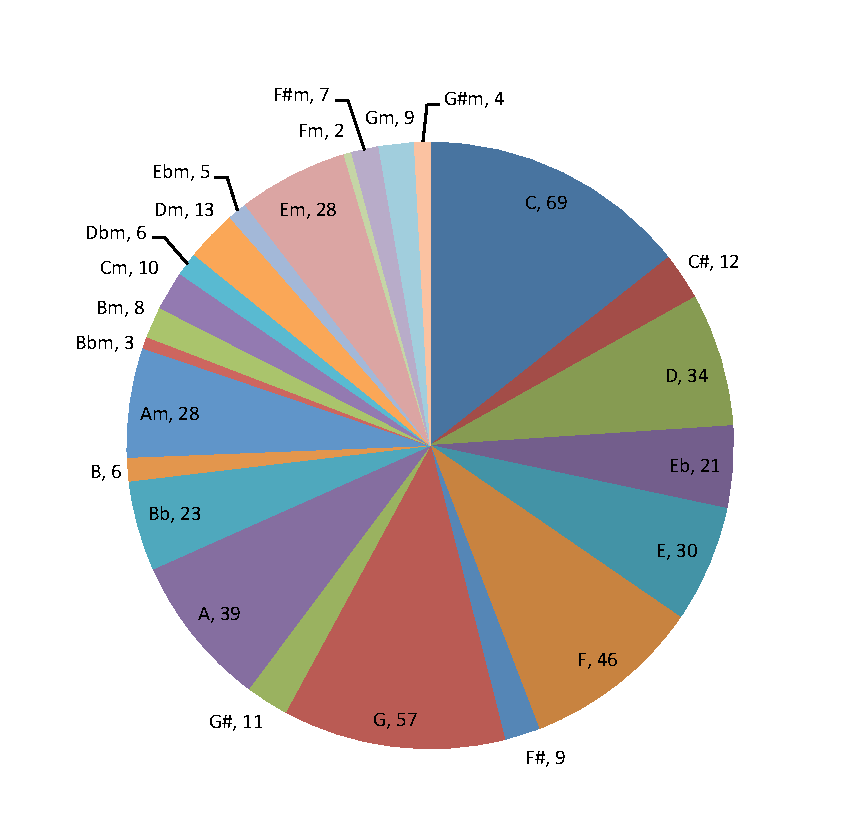
\includegraphics[width=.4\textwidth]{./key_distribution.pdf}
  \caption{\emph{Key distribution of pop melodies}. Every key is represented at least twice in the subset of melodies. In general keys with fewer sharps and flats are more highly represented.}
  \label{fig:key_distribution}
\end{figure}

\begin{table}[]
\centering
\caption{Highly Represented Pop Artists}
\label{tab:data_summary}
\begin{tabular}{@{}lc@{}}
\toprule
Artist & \# of songs\\ \midrule
beatles	& 28 \\
elvis presley	& 13 \\
kiss	&	11 \\
madonna	&	8 \\
eagles	&	6 \\
aerosmith	&	6 \\
elton john	&	6 \\
u2	&	6 \\
beach boys	&	5 \\
michael jackson	&	5 \\
pink floyd	&	5 \\
bobby vee		&	5 \\
adele	&	5 \\
queen	&	4 \\
kinks		&	4 \\
\end{tabular}
\end{table}

\subsection{Implementation}

We compared the accuracy of 4 traditional and 5 machine learning methods on the task of inferring key signature for pop melodies. For the machine learning methods, we used 10-fold cross validation for training and testing.

\emph{Minimize Accidentals By Count}. This algorithm represents the common theory that the best key is that which minimizes the number of resulting accidentals.

\emph{Minimize Accidentals By Duration}. Similar to the previous method but finds the key which minimizes the total duration of accidentals.

\emph{RMSE of Pitch Count Profiles}. Similar to the method followed by \cite{krumhansl2001cognitive} and others, we generated pitch profiles. Rather than generate profiles for each major and minor key, we chose to generate a single profile for all major keys and a second for all minor keys. This decision is based on the assumption that the variation in pitch distribution varies very little (if at all) as compared to the distributional variation between the major and minor modes. Major and Minor mode pitch profiles were generated from the pitch counts in training instances normalized to either the C major or A minor keys depending on the whether the instance was major or minor. A pitch profile is created for each test instance, transposed into each of the 12 possible keys. Each transposed profile is compared to both the major and minor generic pitch profiles using root mean squared error (RMSE). The transposed pitch profile and the major/minor pitch profile with the minimum RMSE value are used to infer key and modality.

\emph{RMSE of Pitch Duration Profiles}. Similar to the previous method but pitch profiles are generated from pitch durations rather than mere counts (see Figure~\ref{fig:pitch_profiles}). 

n\emph{-gram Models}. An n-gram model calculates the probability of the next token given some context window of length \emph{n}. These probabilities are learned from the sequence of notes in the training instances and then used to calculate the probability of note sequences in the test instances. We trained \emph{n}-gram models for values of n from 1 to 5, using Laplace smoothing and a pseudocount alpha value of 1. For each value of \emph{n} a single \emph{n}-gram model was trained for melodies in major keys and another for melodies in minor keys. Probabilities were normalized across both models. Training instances were than transposed and scored by each trained model. The transposition and model which maximized the probability of the training instance determined the key and modality.

In addition to the methods described above, we also report accuracy from three other sources. The baseline accuracy represents the approach of always guessing the most common class. MIDI Annotations refers to the key signature that was originally given in the MIDI file (if any was provided).

Lastly we report the accuracy of a third-party MIDI-reader called MuseScore. Our interest in this problem was initially sparked by the need to normalize lyricized pop music data for compositional analysis. The most ready source for data of this type was found to be karaoke files in MIDI format (also referred to as the KAR format). Insofar as MIDI is a format concerned primarily with generating audio, many such files fail to include (accurate) information about key or time signature, thus motivating the need to infer this information from the notes themselves. This functionality is built in with varying success to many programs which render MIDI files as sheet music. MuseScore (version 2.0.3) is one such program and we include the accuracy of MuseScore's inferred key-signature in our results for comparison. 

\begin{figure}
  \centering
 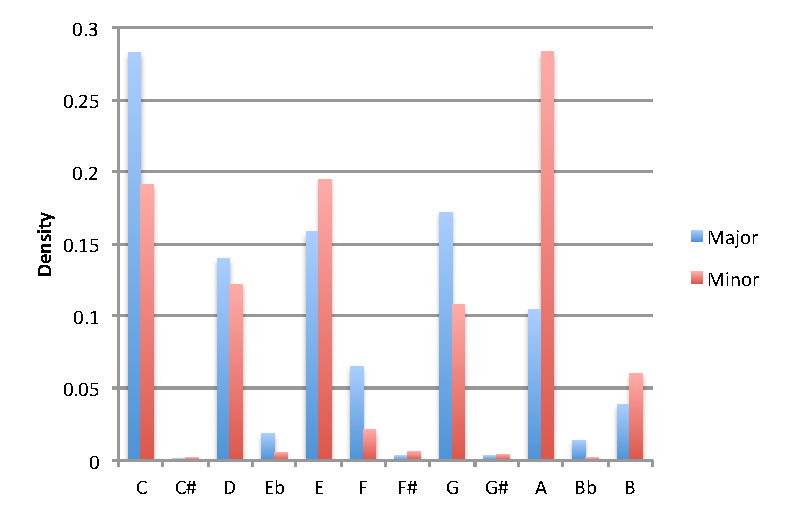
\includegraphics[width=.5\textwidth]{./PitchProfilesWeighted.pdf}
  \caption{\emph{Weighted Major/Minor Pitch Profiles}. Profiles are based on the duration of pitches in each of the major and minor modes. Profiles for major keys (blue) have been normalized to C major and those for minor keys (red) to A minor. Note that the A pitch is relatively more frequent for minor keys (where it functions as the tonic) than for major keys (where it functions as the 6th from the root). Likewise the G pitch is relatively more frequent for major keys (where it functions as the dominant) than for minor keys (where it functions as the 7th from the root).}
  \label{fig:pitch_profiles}
\end{figure}

\section{Results}

Results are shown in Table~\ref{tab:results}. We report accuracy both for inferring the key and for inferring the key signature. Inasmuch as key signature is a more generic classification of key (e.g., C major and A minor both have a key signature with no flats or sharps), accuracy for key signature will always be better than accuracy for key.
\begin{table}[]
\centering
\caption{Key Finding Accuracy for Pop Melodies}
\label{tab:results}
\begin{tabular}{@{}lll@{}}
\toprule
Method & Key & Key Signature \\ \midrule
Baseline (C)	&	0.144 	&	0.202 \\
MIDI	Annotations		&	n/a		&	0.483 \\
MuseScore	&	n/a		&	0.746 \\ \midrule
Minimize Accidentals	 by Count	&	0.494 &		0.660 \\
Minimize Accidentals	 by Duration	&	0.490 &		0.665 \\
RMSE of Pitch Count Profiles	&	0.606	&	0.796	\\
RMSE of Pitch Duration Profiles	&	0.613	&	0.765	\\ \midrule
Unigram model    	&	0.629	& 0.815       \\
Bigram model		&	0.654	&	0.883	\\
Trigram model		&	0.679	&	0.883	\\
4-gram model		&	\emph{0.729} &	\emph{0.896}	\\
5-gram model		&	0.700 &	0.885              \\ \bottomrule
\end{tabular}
\end{table}

\section{Discussion and Conclusion}

Normalizing to a common key really only requires that we identify the key signature for a composition without regard for whether the key is the major key associated with the key signature or its relative minor. We chose to model the major and minor separately based on the hypothesis that the melodies that each produces would be sufficiently different to warrant creating individual profiles.The key inference methods which minimize the frequency of accidentals show the most dramatic improvement because these methods inherently fail to provide a way of distinguishing between a major key and its relative minor.

We encountered several challenges unique to the pop music domain. Songs based on blues scales often include the flat seventh (which would suggest a key a fifth below the actual tonic) or both the major and minor third. Hard rock songs often exclude the third all-together, making it difficult to infer whether a major or minor key signature is more accurate. These confounding influences are reflected in the confusion matrices for classifications of songs in these genres (see Figure~\ref{fig:confusion_matrix}).

\begin{figure*}
  \centering
 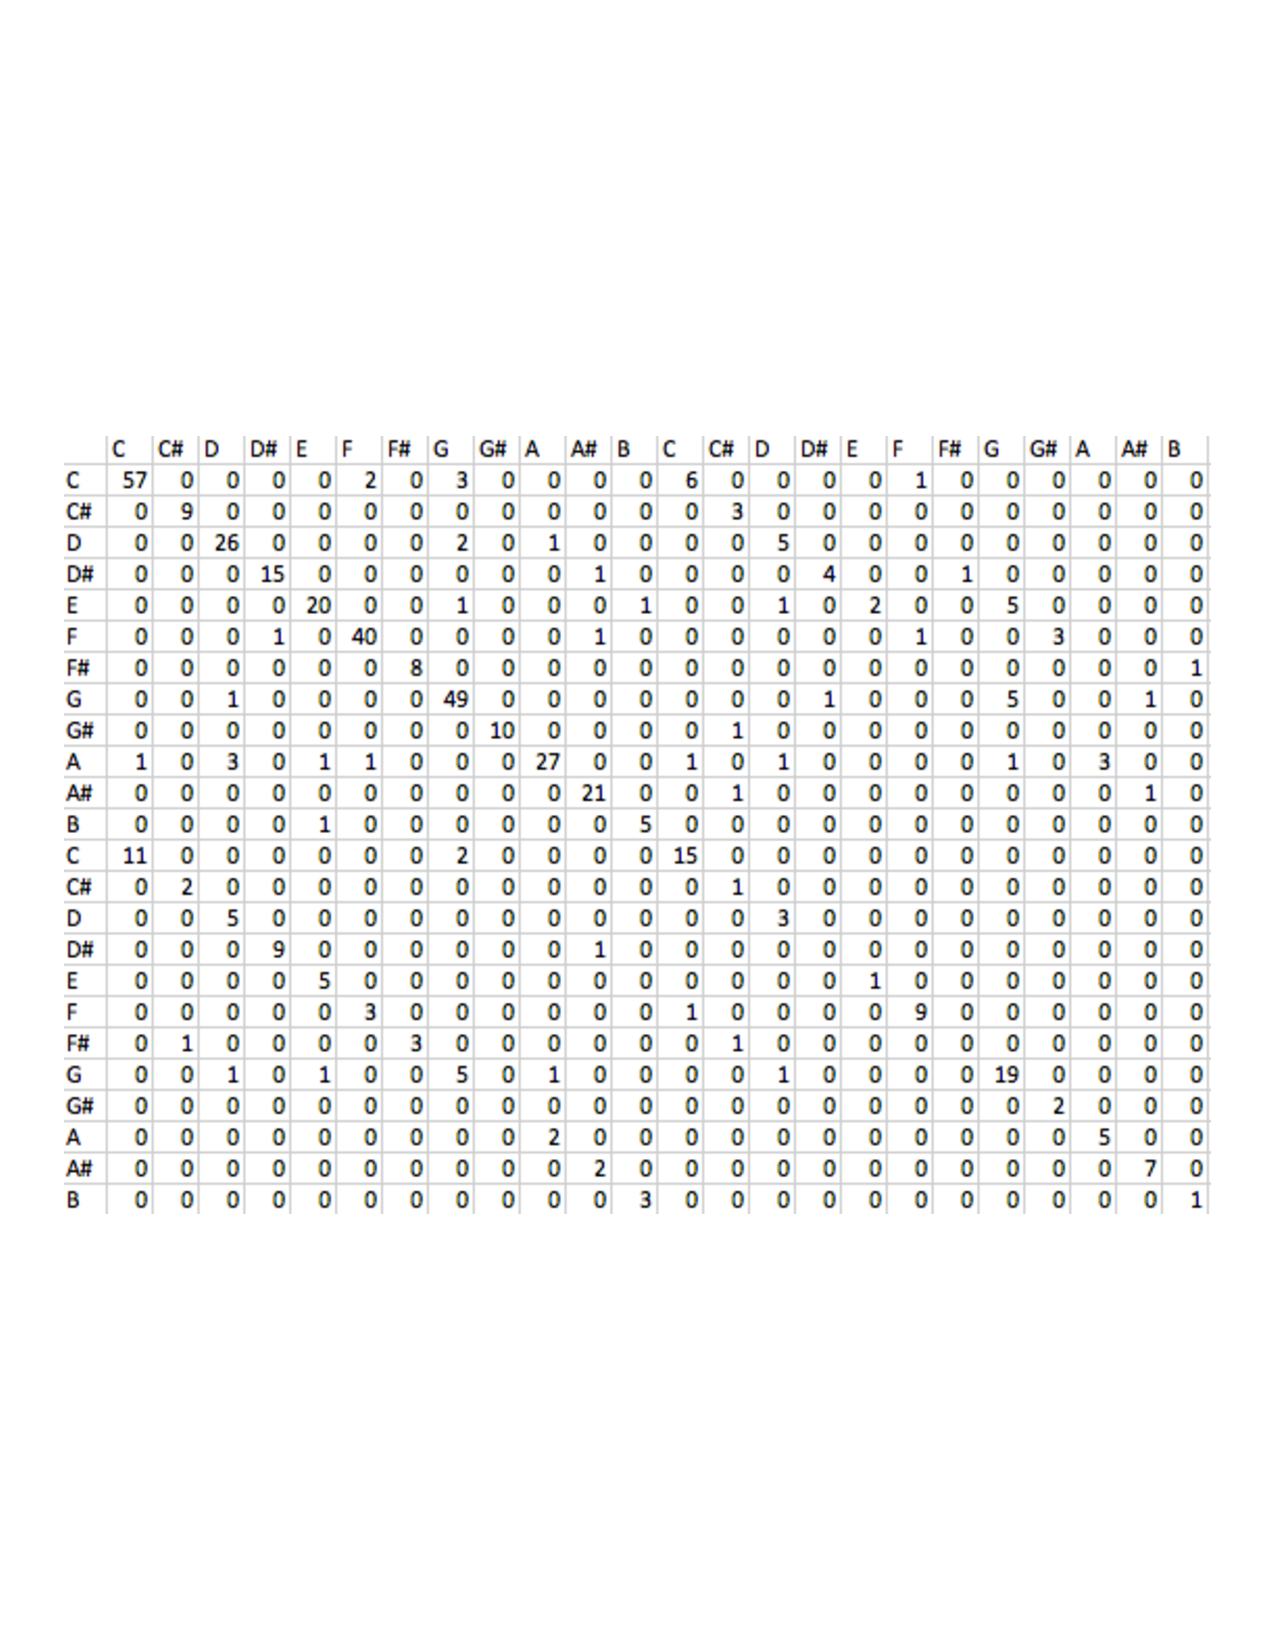
\includegraphics[width=\textwidth]{./confusion_matrix.pdf}
  \caption{\emph{Confusion Matrix for 4-gram model}. Much of the mis-classification confuses major and minor modes for the same key. In cases such as hard rock which use open fifths and exclude the third completely the mode (i.e., major or minor) is difficult to establish.}
  \label{fig:confusion_matrix}
\end{figure*}
``quote''
As regards the \emph{n}-gram models, we note that the unigram model is essentially equivalent to a pitch profile rendered as an applied probability distribution, and thus it seems reasonable that it should perform about on par with the RMSE of Pitch Count Profile method.

We increased the value of \emph{n} until we observed a decrease in accuracy. As is typical of \emph{n}-gram models, as \emph{n} increases, the model begins to essentially memorize more than can be generalized from the training data to the test data at which point the differences between instances become as significant as the differences between the key classes.

It is important to note that although our best accuracy on key-finding (.729) is significantly below the values reported by studies mentioned in the related works, the task of inferring key from melody is significantly more challenging than inferring key from songs which include harmony. It should also be considered that human listeners that are familiar with a melody may more accurately infer key from having familiarity with the harmony also. We therefore express confidence in the reported accuracies of these models.

Our results suggest that considering pitch counts or durations is less effective than a model which considers the sequence of pitches. This agrees with our intuition insofar as many pop songs spend the bulk of their duration modulating through chords which are not the root and may not even be closely related to the root. Notions of resolution and finding where the song ``lands'' inherently suggest that the contour and progression of the notes matters more than their frequency. The key is often most clearly defined at the beginning and ends of musical phrases or the beginning and end of the song itself. Whereas the method of counting note frequencies fails to give higher weight to these defining regions of the melodic passage, this information is embedded within the probabilistic framework of \emph{n}-gram models.

We find the superior accuracy of \emph{n}-gram models to the MuseScore key-signature inference model to be particularly promising inasmuch as it suggests that an \emph{n}-gram model might be used to improve the state of the art in industrial MIDI-reading software.

As regards key inference from monophonic pop melodies, we find that machine learning methods (\emph{n}-gram language models in particular) perform better than traditional key-finding algorithms, though both improve upon baseline accuracy. In the future we hope to evaluate how well unbiased human listeners would perform on the same task. We also envision developing a framework for detecting key \emph{changes} in pop melodies and for normalizing unlabeled melodic data for compositional analysis. 

\bibliographystyle{aaai}
\bibliography{bibfile1}

\end{document}
